\documentclass[superscriptaddress,twocolumn,pre]{revtex4}

\usepackage{ifthen}
\newboolean{pnas}
\setboolean{pnas}{false}

\usepackage{amsmath}
\usepackage{amsfonts}
\usepackage{amssymb}
\usepackage{mathtools}
\usepackage{graphicx}
\usepackage[T1]{fontenc}
\usepackage[utf8]{inputenc}
\graphicspath{{images/}}
\usepackage{color}
\usepackage[pdfstartview=FitH,
            breaklinks=true,
            bookmarksopen=false,
            bookmarksnumbered=true,
            colorlinks=true,
            linkcolor=black,
            citecolor=black,
            urlcolor=black,
            pdftitle={Peptidome},
            pdfauthor={Andreas Mayer},
            pdfsubject={}
            ]{hyperref}
\newcommand{\B}{\boldsymbol}
\newcommand{\ud}{\mathrm{d}}
\newcommand{\<}{\langle}
\renewcommand{\>}{\rangle}

\def\(({\left(}
\def\)){\right)}                       
\def\[[{\left[}
\def\]]{\right]}

\newcommand{\AM}[1]{{\color{blue}#1}}

\begin{document}

\title{The statistical ensemble approach to self/non-self immune discrimination}
%\author{Andreas Mayer}
%\author{Quentin Marcou}
%\author{Warren James}
%\author{Christopher Russo}
%\author{William Bialek*}
%\author{Benjamin D Greenbaum*}
\date{\today}

\begin{abstract}
The immune system needs to distinguish molecular features of pathogens from those found in an organisms' own proteome. A naive but universal way to discriminate would be to have an immune system that can uniformly recognize any possible non-self peptide while "white-listing" every self peptide that should not elicit a reaction through negative selection. This historically prevailing view has been challenged in recent decades for the T cell system by experiments showing many self-peptides are not entirely eliminated, but either do not make recognizable antigens or are suppressed via regulatory machinery, and that cross-reactive T-cell receptors can be highly non-specific. The implication is that the immune system has adopted a fundamentally different evolutionary strategy than was thought which needs to be better understood. We characterize self and pathogen proteomes as statistical ensembles. Probabilistic models reveal how both universal and phyla-specific constraints on protein evolution shape the statistics of both proteomes, allowing us to quantify to what extent proteome ensembles differ systematically, and posit that the immune system has evolved to maximize the likelihood of recognition based on peptide statistics, since evolution is unlikely to develop strategies to combat pathogen features an organism never encounters. We propose the immune system evolved to leverage these statistical differences for efficient pathogen defense. Finally, we compare predictions from our efficient immune strategy to what is known about epitopes recognized by the immune system. In doing so our theory predicts two established features of the immune system: the abundance of pathogen peptides that are closer to self than would be expected from the uniform model and the immunodominace of a small set that drive immune recognition. The success of our approach in predicting these two fundamental features of immune recognition implies the immune system evolved to leverage statistical differences rather than focus on proteins that are "far from self". 
\end{abstract}

\maketitle

\section{Introduction}

A key question in quantitative immunology is how the immune system distinguishes foreign antigens from self-antigens. There is one view of adaptive immunity in which both self and non-self antigens are random samples from a common (and essentially uniform) universe of peptides of a given length. Discrimination is then achieved primarily on the basis of white-listing: thymic negative selection acts to get rid of those T cells that are reactive to self, leaving everything else as a potentially, and equally, recognizable foreign antigen. If the two types of antigens are instead drawn from different distributions, then some regions of peptide space will be much more likely to be self and some much more likely to be non-self. Over evolutionary timescales the recombination machinery could have evolved to bias the immune repertoire towards recognizing antigens that are more statistically unlikely to arise from the human proteome. For instance, as  host and pathogen may use different types of proteins in different types of environments, the amino acid and nucleic acid distributions needed for proper functioning of a protein might differ. Alternatively, however, coevolution of pathogens with their hosts might select for pathogens that have a more similar distribution of peptides to their host than they would otherwise have by chance. The ability to address these issues experimentally has drastically changed our view of the T cell recognition machinery over the past decade \cite{Davis2015, Birnbaum2014}. It is clear thymic selection eliminates self reactive T cells only partially and there are many self-reactive T cells in the blood that survive thymic selection, only to be suppressed by peripheral regulation. Moreover, T cell recognition is non-specific, as a cross-reactive T cell maybe be capable of recognizing many hundred peptides. It is therefore clear that self-peptides are eliminated only partially, likely in a biased manner, and that a cross-reactive T-cell receptor repertoire engages in negative selection only partially. 

The question of through what lens the immune system "sees" the world has renewed urgency in the context of cancer immunotherapy and the design of antigen based RNA vaccines for SARS-CoV-2 \cite{Luksza2017,Balachandran2017,Richman2019}. For instance, as it has become clear that the immune system is capable of recognizing peptides that differ by a sinle mutations in a tumor (referred to as neoantigens), which sort of antigens are more easily recognizable by the immune system and which self-antigens are more likely to be tolerized has become a critical question. If there is a bias present in what makes a good antigen, this would aide {\it in silico} predictions of response and the development of targets for next generation therapies, such as anti-tumor vaccines. Here we revisit the often tacit assumptions about how evolution of the immune machinery shapes antigen prediction. In particular, there is a prevailing view that detecting neoantigens is hard because they are often similar to self, and that pathogen associated antigens are far from self. If pathogens are generically very different from self then why would the immune system have evolved the capability of resolving small differences as is the case for neoantigens? We question the prevailing view by showing that the primary deviations away from a uniform distribution over oligomers are shared between between self and non-self peptides. That is, biases exist in both peptide and antigen distributions, but those biases are actually shared. 

%Previous immuno-peptidome analyses have focused on similarity between self and non-self peptides. Work by Claverie and co-workers \cite{Claverie1988} and later by Burroughs, De Boer, and Kesmir \cite{Burroughs2004} demonstrate that the number of shared nonamers decreases with evolutionary distance. The later work discusses some possible slight preference of the antigen processing pathway for non-self antigens. In a follow up work an overlapping set of authors build a tool for immunogenicity prediction based on small differences in amino acid usage in recognized epitopes \cite{Calis2013}, as well as discuss potential large holes created by self-tolerance \cite{Calis2012a}. A more recent follow up by Wortel et al. \cite{Wortel2018} shows that self and foreign peptides are largely similar (much more similar then words from different languages). They argue that under these conditions thymic selection should minimize the co-occurrence of similar self-peptides for efficient self/non-self discrimination based on negative selection. The emerging view would suggest that the immunogenicity of an antigen, via T cell reactivity, is related to how untypical it is given the normal distribution of the human proteome, rather than precision whitelisting. Recent works has found productivity in mutation derived neoantigen immunogenicity prediction both by incorporating distances to immunogenic viral peptides \cite{Luksza}, and distance from the self-proteome \cite{Vonderheide}. In cancer immunology \cite{Walz2015} it has also been known for sometime that immune activation can be achieved not just by neoantigens but also by large changes in protein abundance, such as those arising from epigenetic dysregulation. While mutation derived neoantigens have been implicated in response to checkpoint blockade immunotherapy, they are not the only source of immunogenicity \cite{XXX}. As such, bias towards unlikley peptides would account for both sequence and expression based discrimination.

%Even a single proteome contains a great deal of data. The approximately 20000 genes times 1000 amino acids per gene on average gives $2 \cdot 10^7$ possible {\it k}-mer peptides, when not accounting restrictions on which can be processed and presented \cite{Luksza}. This also implies that most 5mers will still be represented in the proteome, as there are only about $20^5 = 3.2 \cdot 10^6$ possible 5mers. As a consequence, small changes in amino acid usage can lead to larger changes in the relative likelihood of longer stretches of otherwise random sequences: consider a 10\% difference for single amino acids than a random 8mer has a log-likelihood ratio of $1.1^8 \approx 2.15$. Even larger likelihood ratios are expected for long {\it k}-mers once pairwise or higher-order correlations are considered  \cite{Schneidman2006}. In that sense, the ability to capture features of genuine antigens would come from an adequate statistical model that captures typical self-peptides. Karlin and Bucher \cite{Karlin1992} have shown the existence of pairwise correlations in amino acid usage and discuss various structural reasons for these correlations. Peer et al. \cite{Peer2004} have shown that amino acid and oligopeptide compositions differentiate among phyla, which implies one can construct models of self-peptide that are not simply random, and follow up work has shown similar conclusions \cite{Bogatyreva2006}. On the other hand \cite{Lavelle2009} claim that generally 4mers and 5mers do not show large deviations from random models when taking care to remove bias by large protein families, implying the diversification of and selection upon these families account for most organism specific difference. On a more general level the question which structural constraints restrain the evolution of amino acid patterns has received attention for a long time \cite{Turjanski2018}. Random strings of amino acids do not yield valid, folding proteins, but amino acid strings of natural proteins are hard to distinguish from random, other than by deviations from uniform in individual amino acid frequencies that seem to be governed by amino acid mass \cite{BenAlbert}.

Given that it is possible at all to evolve a system to discriminate small differences, we propose an efficient immune defense should focus on deviations from "more likely" regions, which the immune system can learn the statistics of from the self-proteome. To capture these effects, we start by establishing an ensemble model of the self-proteome, demonstrating that most long peptides are random, other than single amino acid biases and a small amount of comparatively weak correlations. We build a maximum entropy distribution constrained to reproduce the amino acid frequencies and the correlations between pairs of amino acids a given distance apart (as we consider random substrings the distribution should only depend on absolute distance).  In doing so, we construct a theory of immune recognition whereby the species specific biases in the self-peptidome are leveraged to find deviations from the self-distribution by pathogens. As pathogens, specifically viruses, have higher diversity that the self-proteome, yet need to interact with its internal machinery, we argue an immune model based on deviation from the "biased self", rather than trying to target pathogens uniformly and whitelisting, is optimal and show how the observation of peptides close to self and immunodominant antigens result as a consequence. 

\section{Results}

\subsection{Discriminability of host and pathogen peptides}


\begin{figure}
    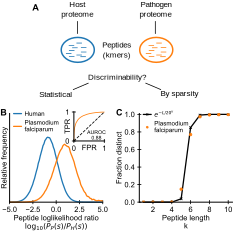
\includegraphics{classifier}
        \caption{{\bf Two views on the discriminability of host and pathogen peptides.} (A) The adaptive immune system interacts with peptides derived from either host or pathogen proteins. How discriminable are peptides drawn from different proteomes? (B) Histograms of loglikelihood ratios for 9mers drawn randomly from a pathogen (Plasmodium falciparum) or human proteome. The likelihood is defined here simply by the average amino acid frequencies in both sets of sequences. (B, inset) Sensitivity (true positive rate - TPR) vs. specificity (false positive rate - FPR) tradeoff curve for a binary classification based on the likelihood ratio. (C) Fraction of pathogen peptides of different length that are distinct from all peptides from the host.
    \label{figclassifier}
    }
\end{figure}

We aim to understand how the biophysics of protein statistics might have shaped the evolution of adaptive immune recognition (Fig.~\ref{figclassifier}). Classification between two sets of sequences can be achieved based on differences in sequence features. Such a type of classification underlies all machine learning classification algorithms: given a training set with items of each class the algorithms aim at generalizing by inferring statistical features that allow discrimination. Alternatively, if the set of sequences is finite and sparsely covers the space of all possible sequences, discrimination can also be achieved by memorization, as would be the case by whitelisting peptides from the host proteome by a combination of negative selection and induction of regulatory cells. To anchor our further explorations we here analyze the ability of both strategies to classify peptides of a given length drawn at random either from a pathogen proteome or the host proteome.

To illustrate when discrimination exploiting finiteness is possible we analyze how the fraction of peptides that are found only in a pathogen protein, but in none of the host proteins depend on the peptide length $k$. Intuitively, the critical value of $k$, beyond which most pathogen peptides are not to be found in the host proteome, is set by a comparison of the length $L$ of the host proteome to the exponentially increasing number of different kmers $20^k$. Simple combinatorics based on random sequences matches predicts that a random pathogen peptide is not present among the $\sim L$ possible host peptides with a probability $e^{-L/20^k}$ (SI Text~\ref{secsequencematching}). This prediction agrees qualitatively with the empirical data calculated from the Plasmodium falciparum proteome (the parasite causing Malaria) with respect to the statistics of human host proteins(Fig.~\ref{figclassifier}C). Quantitatively, there is a small difference, with the empirical relationship being less steep as a function of $k$ owing to non-randomness in the sequence space coverage. From both theory and data we find that a majority of peptides are distinct for peptides of length $k\geq6$ (orange dots, Fig.~\ref{figclassifier}C), thus setting a minimal length scale needed for this mode of immune discrimination.  

To illustrate statistical discriminability we describe the statistics of each proteome using an independent site model, only taking into account differences in average amino acid usage between proteomes. These models assign a probability $P(\B \sigma)$ to each peptide $\B \sigma$ of the form $P(\B \sigma) = \prod_{i=1}^k P(\sigma_i)$. Given probability distributions $P_H(\B \sigma)$ and $P_P(\B \sigma)$ for the host and pathogen, respectively, we can calculate a likelihood ratio as a measure based on which to classify peptides. Fig.~\ref{figclassifier}B shows the distributions of likelihood ratios for peptides of length $k=9$ amino acids for the same host/pathogen pair considered before. By choosing an appropriate cutoff one can turn the likelihood ratio into a binary decision of whether a given peptide originates from one of the two proteomes. We visualize the accuracy with which such a classifier discriminates between host and pathogen peptides as a function of different threshold values in the form of a sensitivity-specificity tradeoff curve (Fig.~\ref{figclassifier}B inset). Here, sensitivity is defined as the fraction of foreign peptides correctly classified as such, and specificity as the fraction of false positives from the host proteome. Quantifying the discrimination accuracy using the area under this curve confirms a substantial statistical discriminability (AUROC = 0.89), although discrimination is not perfect as is clear from the overlap of the distributions of likelihood ratios.

%However, this measure focuses on the overall discriminability, while the immune system might instead make a decision bases on only a few peptides that are particularly easy to discriminate. To assess the accuracy of such a classification strategy, it is particular convenient to display the data in the form of a precision-recall curve (Fig.~\ref{figclassifier}C,F).

Many questions remain open from our analyses so far, and will be answered in the following. First, is there higher order statistical structure in peptide space that might increase discriminability? Second, to the extent that there are statistical differences, do they generalize across pathogens? Third, what are the implications of the above statistical analyses for the evolution of immune recognition?


\subsection{A statistical physics framework to quantify peptide statistics} 


\begin{figure*}
    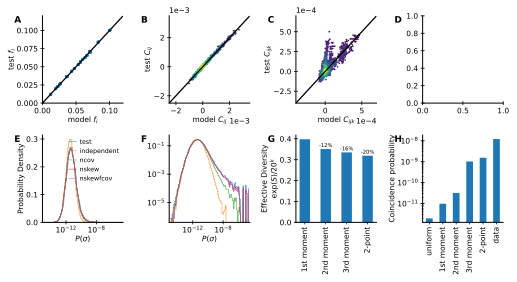
\includegraphics{maxent}
        \caption{{\bf Maximum entropy models of peptide statistics.} A maximum entropy model with third order compositional constraints and second order pairwise constraints on amino acid covariations captures the statistics of the human proteome. (A-C) Comparison of connected correlation functions in the test set with model predictions. (D,E) Density of states relative to the full energy function of models with different types of constraints. (G) Reduction in effective diversity of the peptide distribution resulting from imposing different constraints. The cumulative percentage reduction of effective diversity relative to the first moment model is indicated for each of the nested models. (H) Probability of coincidences in the different models, $\sum_{\B \sigma} P(\B \sigma)^2$.
    \label{figmaxent}
    }
\end{figure*}

We propose to use a maximum entropy framework a, and will be answered in the followings a principled way to include increasingly detailed statistical structure into a series nested models of peptide statistics. Using this approach we constrain a set of statistical observables $\langle f_\mu(\boldsymbol \sigma)\rangle$ to equal their empirical values $\bar{f_\mu}$, while otherwise keeping the probability distribution as random as possible. Mathematically, this means choosing the probability distribution to maximize the Shannon entropy
\begin{equation}
    S[P(\B \sigma)] = - \sum_{\B \sigma} P(\B \sigma) \log P(\B \sigma),
\end{equation}
subject to the normalization constraint $\sum_{\B \sigma} P(\B \sigma) = 1$, and constraints that enforce the equality of modelled and empirical observables
\begin{equation}
    \langle f_\mu(\boldsymbol \sigma)\rangle = \sum_{\boldsymbol \sigma} P(\boldsymbol \sigma) f_\mu(\boldsymbol \sigma) = \bar{f_\mu}.
\end{equation}
Optimizing with respect to the normalization constraint yields a Boltzmann distribution of the form,
\begin{equation}
    P(\boldsymbol \sigma) = \frac{1}{Z} \exp\left[ -E(\B \sigma) \right],
\end{equation}
where
\begin{equation}
 E(\B \sigma) = \sum_{\mu=1}^K \lambda_\mu f_\mu(\boldsymbol \sigma),
\end{equation}
is a sum of terms involving each constraint, which is called the energy in statistical mechanics, and 
\begin{equation}
    Z = \sum_{\B \sigma} \exp \left[ - E(\B \sigma) \right]
\end{equation}
is a normalization factor, called the partition function.

We fit the parameters $\lambda_\mu$ to the data using Boltzmann machine learning \cite{Ackley1985}. In short, we iteratively estimate $\langle f_\mu(\B \sigma)\rangle$ using Monte Carlo sampling for a given set of model parameters and then update parameters to minimize the discrepancy between estimated and empirical observables (Materials and Methods).
%To assess potential overfitting we split the dataset into a training and a test set of equal size. We calculate the average of observables used in the fitting on the training set, but compare model predictions against the test set.
We have constructed a hierarchy of such models to assess the significance of different constraints. We have found that a satisfactory model of 9mers drawn from the human proteome is provided by fitting the moments of the amino acid composition of peptides up to third-order, together with distance-dependent 2-point couplings. Taken together, these constraints produce a model that recapitulates key statistical features of the data (Fig.~\ref{figmaxent}). By construction, the fitted model reproduces the average frequencies $f_i(\alpha)$ of finding amino acid $\alpha$ at position $i$ (Fig.~\ref{figmaxent}A), as well as the connected two point correlation function $C_{ij}(\alpha, \beta) = f_{ij}(\alpha, \beta) - f_i(\alpha) f_j(\beta)$ (Fig.~\ref{figmaxent}B). As a test of the model, we compare predicted and empirical connected three point correlation function $C_{ijk}(\alpha, \beta, \gamma) = f_{ijk}(\alpha, \beta, \gamma) - f_{ij}(\alpha, \beta) f_k(\gamma) - f_{ik}(\alpha, \gamma) f_j(\beta) - f_{jk}(\beta, \gamma) f_i(\alpha) + 2 f_i(\alpha) f_j(\beta) f_k(\gamma)$ (Fig.~\ref{figmaxent}C) and find good agreement. Moreover, the density of states is self-consistent between model and data (Fig.~\ref{figmaxent}E,F).
%We note that the model does not include any position dependence, as the data is by construction translation-invariant except for edge effects arising from both ends of the protein. 

To quantify how different constraints reduce the diversity of the ensemble of peptides, we calculate the entropies $S[P(\B \sigma)]$ of the modelled distributions using thermodynamic integration (Material and Methods). Defining diversity as an effective number of equally likely peptides (i.e. as the exponential of the entropy), we find that global amino acid usage biases reduce diversity by 60\%, while further constraints collectively reduce diversity by an additional 20\% (Fig.~\ref{figmaxent}G). While this reduction in diversity is relatively modest, the inclusion of higher-order constraints is important for some observables: For example, we find that the probability with which two randomly drawn peptides coincide increases by orders of magnitude when including the additional constraints (Fig.~\ref{figmaxent}H). Note that the probability of a coincidence is equal to $\sum_{\B \sigma} P(\B \sigma)^2$, and thus puts larger weight than the entropy on the upper tail of probabilities. The increase of coincidences is thus linked to the fatter tail of highly likely sequences in the higher-order models (Fig.~\ref{figmaxent}E,F).

\subsection{Statistical structure of host and pathogen proteomes}

\begin{figure}
    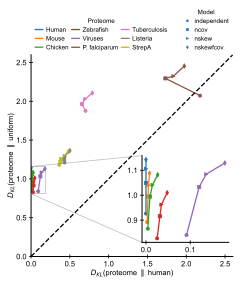
\includegraphics{dkls}
    \caption{Kullback-Leibler divergences between peptide distributions drawn from different proteomes relative to human host peptides and relative to a uniform distribution over all peptides. For each proteome we show the statistical distance calculated according to a nested set of models including a different number of constraints. The inset shows a zoom on the set of proteomes close to the human statistics.
    \label{figdkls}
    }
\end{figure}

We compare here a set of proteomes from model organisms across different branches of jawed vertebrates: Human and Mouse as two examples of animals, Chicken as an example of a bird, and Zebrafish as an example of a jawed fish. We also compare them against a set of pathogen proteomes: A collection of human viruses (individual viral proteomes are to small for reliable statistical analyses), a number of bacterial species, as well as parasites (Plasmodium falciparum causing Malaria). For each of these proteomes we fit the same series of maximum entropy models to capture their statistical structure in increasing detail. We then use thermodynamic integration to quantify the statistical distinguishability of each proteome relative to the human proteome in terms of a Kullback-Leibler divergence. The Kullback-Leibler divergence is equal to the expected log-likelihood ratio for drawing a peptide from the pathogen distribution versus the human distribution. 

We find that with a few notable exceptions divergence are small (Fig.~\ref{figdkls}). Different vertebrates have nearly identitical statistical structure. Peptides from human viruses are remarkably close in statistical distance to the human proteome. Bacterial proteomes differ more substantially, but their divergence is still smaller than 1 nat in all cases. The largest divergence is found for the parasite Plasmodium falciparum, which might be a result of the known AT bias of its genome \cite{Hamilton2017}.

We also calculate the divergences with respect to a uniform distribution. We find that natural peptides are substantially easier to differentiate from a completely random kmer than from natural peptides from a different proteome. This shows that a large fraction of biases in primary sequence statistics is shared among proteomes. Analyzing the divergences across the model hierarchy we find that constraints beyond amino acid usage only modestly increase statistical distances. In most cases the inclusion of additional constraints increases the distance from random peptides more than from human peptides, again pointing at a large degree of conservation of these constraints across proteomes.


\subsection{Implications for immune discrimination}

What can we conclude from our prior results? First, overall statistical biases make the distribution of pathogen peptides non-uniform. This implies that an immune system based on targeting all possible 9mers equally would be inefficient. On the other hand we found that the biases between host and pathogen are mostly shared, and statistical discriminability thus low. This implies that the task of discriminating self from non-self purely based on statistical features, without "overfitting", is hard. In the following, we develop a few quantitative ideas building further on these broad insights.


\subsubsection{Statistical bounds for reliable discriminative quorum sensing}

\begin{figure*}
    \begin{center}
    \includegraphics{humanviruses}
    \end{center}
    \caption{Performance of the models as classifiers. (A) Distributions of likelihood ratios for peptides from host and virus proteins. (B) Sensitivity-specificity tradeoff curve for various models. (C) Precision-recall characteristics at a 10-fold excess of self-peptides.
    \label{figmodelclassifier}
    }
\end{figure*}

Given the small Kullback-Leibler divergence we expect only modest performance of using these models as classifiers. Indeed, we find that the distribution of likelihood ratios overlap significantly (Fig.~\ref{figmodelclassifier}A), which leads to a modest average classification performance as assessed by the area under the receiver operating curve (Fig.~\ref{figmodelclassifier}B). However, similarly to how the small reduction in entropy went along with a large increase in coincidence probability, discriminability in the tails is more substantial: for example when focusing discrimination on the top 1\% of most distinguishable viral peptides the precision is roughly four-fold higher using the higher order models than expected by chance, when host peptides are in 10-fold excess. Viral proteome sizes are in the $10^3-10^4$ amino acid range (higher for DNA then RNA viruses). Assuming 10\% of peptides can be presented, the top 1\% corresponds to the top 1 - 10 peptides.

We can also use our theory to quantify under which conditions a quorum sensing strategy can work, i.e. a decision-making strategy relying not on the presence of a single peptide, but $k$ different peptides, simultaneously present on a cell or in a tissue site. While in practice there are likely constraints on how reliably different cells can pool information to coordinate their decision, here we put a theoretical upper bound on the performance of quorum sensing. To this end, we calculate the distribution of cumulative likelihood ratios for $k$ randomly sampled peptides from either the pathogen or host proteome. We then determine the achievable false negative rate by a decision rule at a fixed false positive rate. We find that more than a hundred peptides are needed for reliable discrimination (Fig.~\ref{figquorum}). However, most of the statistical power stems from a much smaller subset of peptides: if, for example, only the top 1\% of peptides with the largest likelihood ratios are considered the number of peptides needed for reliable responses drops substantially to $\sim 10$. This order of magnitude is consistent with the observed immunodominance of a small set of peptides, implying immunodominance may be explained by quorum sensing of peptides at the tail of a pathogens distribution of peptide statistics.
%Layering of additional effects, such as the heterogeneous affinities of different peptides, would only further decrease the number of peptides needed from this theoretical limit. 

\begin{figure}
    \begin{center}
    \includegraphics{quorum_requirement}
    \end{center}
    \caption{How many peptides allow reliable quorum sensing? Achievable false negative rates at a fixed false positive rate $=10^{-3}$ as a function of the number of peptides. Most of the discrimination ability is driven by a smaller subset of most discriminable peptides. The shaded lines show a 1/$x$ scaling for reference. 
    \label{figquorum}
    }
\end{figure}


%Interestingly, the parasite Plasmodium falciparum has the largest observed divergence from the human amino acid usage, . Vaccinia is higher than other viruses, which might attributable to it replicating outside the nucleus of the host cell using its own set of proteins for DNA replication and gene transcription \cite{Tolonen2001}. Mostly the Kullback-Leibler divergences between the doublet distributions are about twice the single site divergences. Notable exceptions are some of the viral proteomes, but this might be due to finite sampling effects biasing the entropy estimates for these small proteomes.

%kUnder the independent model log-likelihoods are additive and thus the average log-likelihood ratio for a kmer is simply k times the calculated single site $D_{KL}$.
%In the limit of large $k$ 
%Chernoff-Stein Lemma!

%\begin{figure}
%    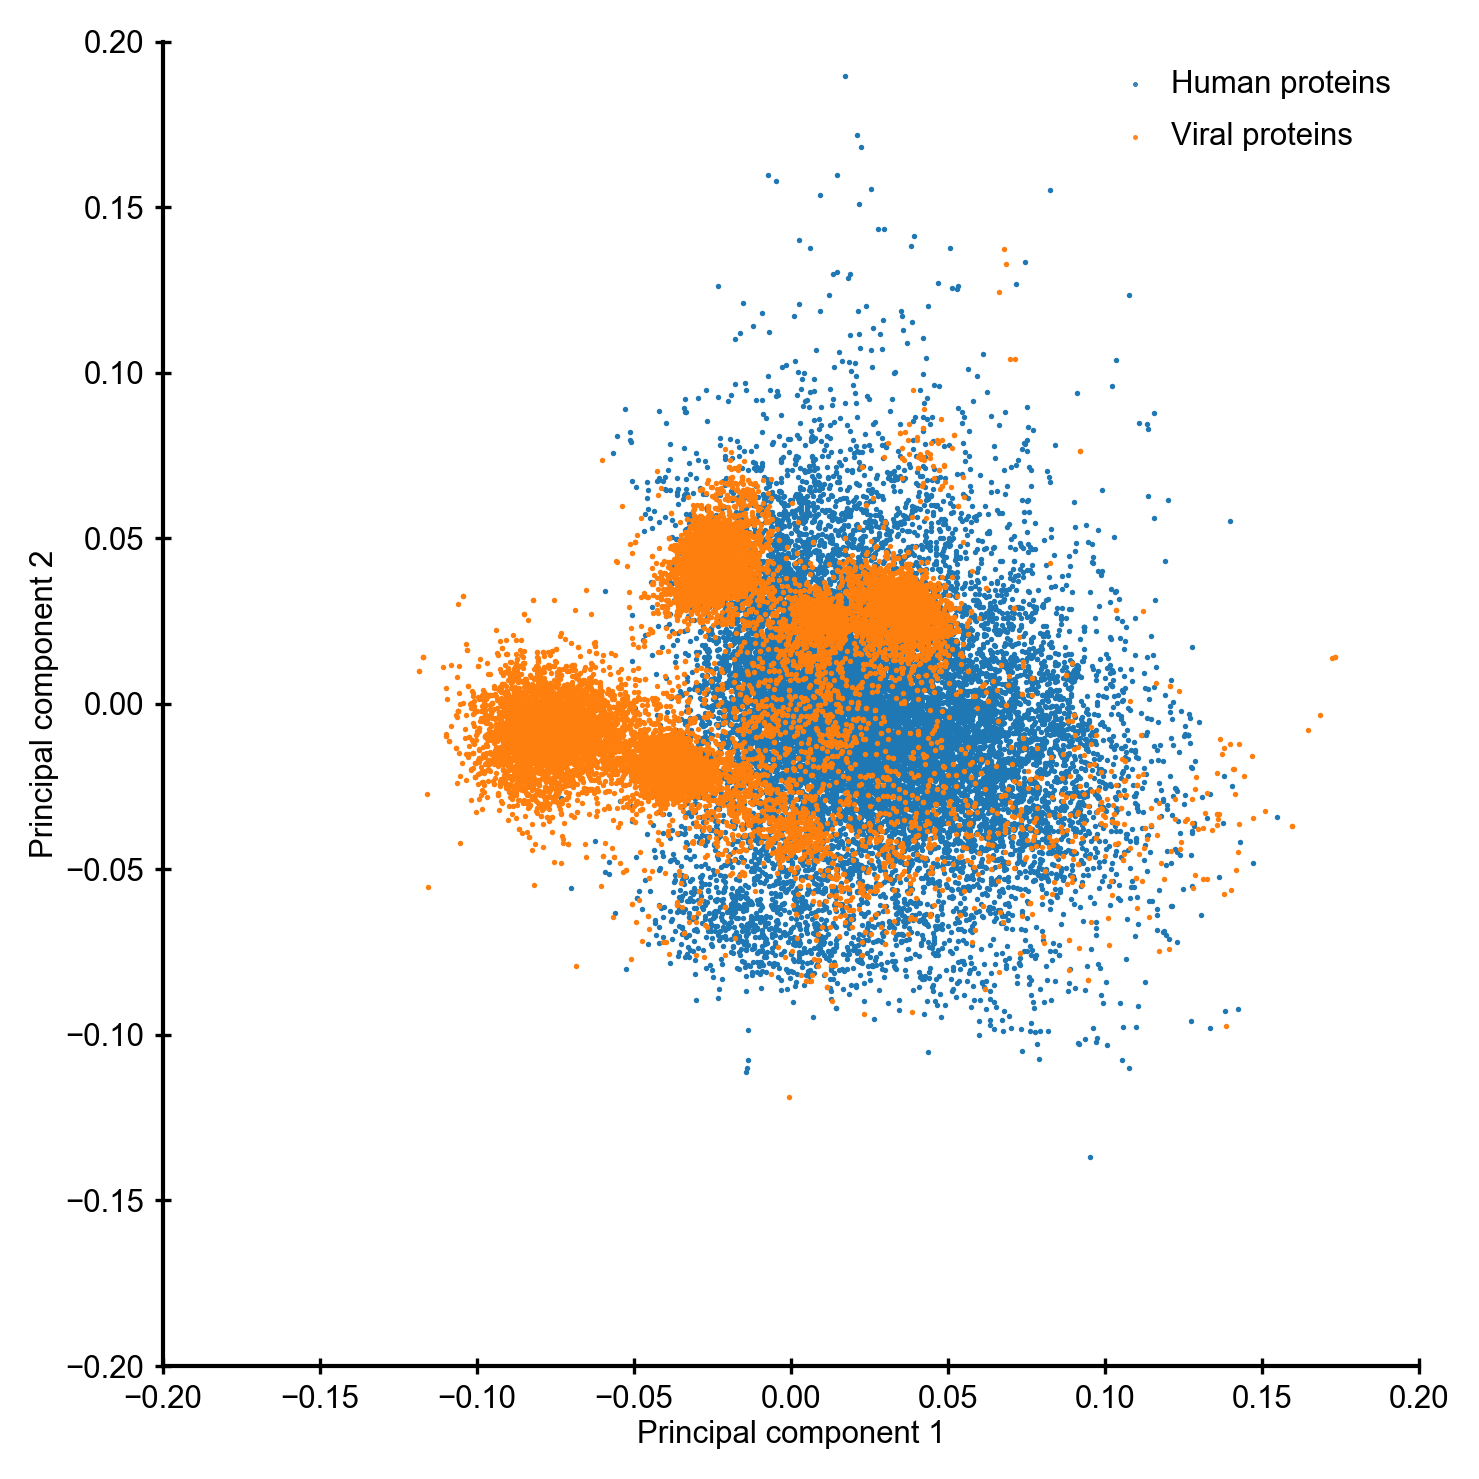
\includegraphics[width=\columnwidth]{viruses}
%    \caption{Likelihood of randomly drawn viral 9mers given a triplet model based on the human proteome statistics. B cell and T cell epitope likelihoods. Interestingly the B cell epitopes are more similar to the human proteome than if they where drawn at random.
%    \label{figviruses}
%    }
%\end{figure}

\subsubsection{Shared sequence biases imply immune epitopes are close to self}

\begin{figure}
    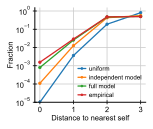
\includegraphics[width=\columnwidth]{neighbors}
    \caption{Distribution of nearest self neighbor distances. For self the distance is calculated to the nearest neighboring peptide, thus excluding any precise alignments.
    \label{figneighbors}
    }
\end{figure}

An important consequence of the shared sequence biases between self and non-self is to make (near-)coincidences between peptides much more likely. To quantify this effect we calculate the distance to the nearest self peptide for a collection of immune epitopes from IEDB (for 9mers). While the reduction in peptide diversity is on the order of tens of a percent, we find the probability of precise coincidences is increased by more than two orders of magnitude compared to the expectation under a uniform model, and near-coincidences differing by a single amino acid are also heavily enriched (Fig.~\ref{figneighbors} red line vs blue line).

\begin{figure}
    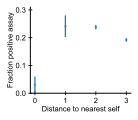
\includegraphics[width=\columnwidth]{iedbposvsdist}
    \caption{Fraction of positive IEDB assay for foreign epitopes as a function of their distance to nearest self peptide.
    \label{figiedbposvsdist}
    }
\end{figure}

To exploit these strongly conserved biases between host and pathogen, immune recognition might focus on generically more common peptides. This could imply that some peptides that are close to self are actually more likely to be recognized than peptides that are very dissimilar. While validation data on immunogenicity remains quite sparse, we can begin to test this assertion using data from the Immune Epitope Database (IEDB). Here we define immunogenicity of an epitope as being associated with a positive assay on immune response. We then calculate the fraction of epitopes at different distances to self that are immunogenic. While epitopes identical to peptides found in the human proteome are somewhat less immunogenic, as expected due to tolerance mechanisms, remarkably, there are many epitopes that differ from self by a single amino acid which are immunogenic. Indeed, the greatest number of immunogenic peptides are only one amino acid away. Moreover, the most dissimilar peptides (distance 3+) are actually recognized with the lowest probability,  implying the immune system preferentially focuses on peptides closer to self, even though farther peptides may be available.


%\subsubsection{Reshaping of the distribution by the presentation pathway}
%
%\begin{figure}
%    \includegraphics[width=\columnwidth]{netmhc_correlations}
%    \caption{How does MHC presentation reshape the peptidome? Every plot shows a histogram of rank correlation coefficients between peptide likelihoods and netMHC predicted binding affinities across all MHC-I types. Binding energy is positively correlated with peptide likelihood under both the human and viral statistics for a majority of MHC-I types, but negatively correlated with the likelihood ratio of viral to human statistics. Thus MHC-binding focuses responses on viral peptides. for a majority of MHC-I types 
%    \label{fignetmhc}
%    }
%\end{figure}
%
%We use neural networks models trained on measured peptide binding to different human MHC molecules to ask how the presentation probability relates to the peptide likelihoods under both the self and foreign statistics. We find that the predicted binding energy is positively correlated with peptide likelihoods under both models for the majority of alleles (Fig.~\ref{fignetmhc}A). Interestingly, sequences that are more likely under the viral than the human statistics are presented more readily (Fig.~\ref{fignetmhc}B).

\section{Discussion}

While we are used to thinking of self and non-self peptide discrimination as either a whitelisting of self-peptides within a uniform distribution of possible antigens, or a set of statistically distinct peptide distributions, we show that self and non-self peptides are generated from similar peptide distribution. As a consequence, when comparing pathogen and host derived peptides, there are not clear statistical differences. The implication is that an efficient immune system would, in the optimal case, focus on peptides that are close to self rather than those that are far from self. Indeed we find empirical support for this prediction in the limited immunogenicity data available to date, supporting the notion that the immune systems preferentially targets epitopes close to self. Moreover, a consequence of these shared biases is that only a small number of antigens are needed for efficient pathogens recognition, offering a novel prediction of immunodominance.

Essentially our findings suggest a "shell model" of immunogenicity - which we describe quantitatively in the Supplemental Information. In such a model the immune system targets epitopes of intermediate likelihoods. A consequence of such a model is a new interpretation of the role of positive and negative selection in thymic selection. Instead of a system where the role of negative selection is strict whitelisting and positive selection solely serves to eliminate T cells that do not recognize any host HLA molecules, our theory suggests that thymic selection may provide a role in training T cells to recognize likely peptides that are close to self, while eliminating only a small subset of peptides that are expressed in somatic tissue.

If further corroborated, this shell model might be of relevance for both vaccine selection and cancer immunotherapy. Mutation derived neoantigens that are only one mutation away from self, might not be that special in the landscape of epitopes the immune system encounters and designing a vaccine whose peptides are far from self might not offer the obvious advantage one might expect. Due to underlying shared biases many more antigens from pathogens are closer to self than naively expected. Hopefully our approach will stimulate a reassement of the approaches evolution might have selected to discriminate self from non-self, while also providing testable prediction that can be used in novel immunotherapies and emerging antiviral strategies.


\section{Material and Methods}

\subsection{Model construction and fitting}

A common choice is to constrain the one and two-point frequencies
\begin{align}
    f_i^\alpha(\B \sigma) &= \sigma_i^\alpha, \\
    f_{ij}^{\alpha\beta}(\B \sigma) &= \sigma_i^\alpha \sigma_j^\beta,
\end{align}
where $\sigma_i^\alpha = 1$ if the amino acid at site i is of type $\alpha$ and zero otherwise.
This leads to a maximum entropy probability distribution that takes the form of a disordered Potts model,
\begin{equation}
    E(\boldsymbol \sigma) = - \sum_{i=1}^L \sum_{\alpha = 1}^{20} h_i^\alpha \sigma_i^\alpha - \sum_{i<j}^L \sum_{\alpha,\beta = 1}^{20} J_{ij}^{\alpha \beta}  \sigma_i^\alpha \sigma_j^\beta.
\end{equation}

Given that many biases are compositional in nature we can also consider a simpler model that only involves a global constraint on the covariation of the total count of amino acids of different types:
\begin{align}
    n^\alpha(\B \sigma) &= \sum_i \sigma_i^\alpha, \\
    n^{\alpha\beta}(\B \sigma) &= n^\alpha(\B \sigma) n^\beta(\B\sigma) = \left(\sum_{i=1}^L \sigma_i^\alpha\right) \left(\sum_{j=1}^L \sigma_j^\beta\right).
\end{align}
This leads to a maximum entropy probability distribution that takes the form
\begin{equation}
    E(\boldsymbol \sigma) = - \sum_{\alpha=1}^{20} h^\alpha n^\alpha -  \sum_{\alpha,\beta = 1}^{20} J^{\alpha \beta} n^\alpha n^\beta,
\end{equation}
i.e. a model that only involves global couplings between amino acids independent of their distance.


The parameters are updated by iterative scaling,
\begin{equation}
    \lambda_\mu^{t+1} = \lambda_\mu^t + \epsilon_\mu^t \log \left( \frac{\langle f_\mu \rangle}{\bar{f_\mu}} \right),
\end{equation}
where $\epsilon_\mu^t$ represents a learning rate (which generally can be coordinate dependent and time-varying).
%The parameters are updated by gradient ascent,
%\begin{equation}
%    \lambda_\mu^{t+1} = \lambda_\mu^t + \epsilon_\mu^t \left(\langle f_\mu \rangle  - \bar{f_\mu}\right),
%\end{equation}
%where $\epsilon_\mu^t$ represents a learning rate (which generally can be coordinate dependent and time-varying).

Once we have fitted the model parameters we can calculate the entropy of the distribution $P(\B \sigma)$. To do so we use the identity
\begin{align}
    S &= - \sum_{\B \sigma}  P(\B \sigma) \log P(\B \sigma),  \\
      &= \langle E(\B \sigma) \rangle - F, \quad F = - \log Z.
\end{align}
The mean energy can be calculated directly from Monte Carlo samples. To calculate the free energy we use thermodynamic integration as follows \cite{Marchi2019b}: We express the energy with respect to a reference energy $E_{ref}(\B \sigma)$ as $E(\B \sigma) = E_{ref}(\B \sigma) + \Delta E(\B\sigma)$, where the reference energy is choosen such that $F_{ref}$ can be calculated analytically. We define the perturbed energy function
\begin{equation}
    E_\alpha(\B \sigma) = E_{ref}(\B \sigma) + \alpha \Delta E(\B\sigma),
\end{equation}
which scales the contribution of the energy beyond the reference model.
To obtain the free energy we use the identity
\begin{equation}
    F(1) = F_{ref} + \int_0^1 \ud \alpha F'(\alpha).
\end{equation}
Note that
\begin{equation}
    F'(\alpha) = - \langle \Delta E(\B \sigma) \rangle_{\alpha},
\end{equation}
which allows us to approximate the integrand by Monte Carlo simulations. We numerically evaluate $F'(\alpha)$ for evenly spaced $\alpha \in [0, 1]$ and calculate the integral by Simpson's rule. Calculating the entropy in this way allows us to determine the reduction in the effective diversity in sequences implied by including different constraints (Fig.~\ref{figmaxent}F). 

\bibliographystyle{apsrev}
\bibliography{library}



\section{A shell theory of immunogenicity?}

\begin{figure}
    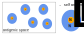
\includegraphics{shelltheorysketch}
    \caption{Sketch of the shell theory of immunogenicity: To be immunogenic an antigen needs to fall outside the tolerance region (orange), but within one of the detectable regions surrounding a self-antigen (blue).
    \label{figshelltheorysketch}
    }
\end{figure}

\begin{figure}
    \includegraphics[width=\columnwidth]{shelltheory}
    \caption{Immunogenicity as a function of the likelihood a peptide in the shell model. The probability of a peptide being immunogenic is defined as the probability of being detectable, but not tolerated. The probability of immunogenicity times the probability of peptides within the pathogen proteome (assumed to be lognormal with $mu = -1.25 k$ and $\sigma = 0.3 k$ with $k=9$) gives a hypothetical expected distribution for the epitopes, which is clipped at both ends.  
    \label{figshelltheory}
    }
\end{figure}

How likely is it that a peptide will be close enough to a self-peptide to be tolerized? How likely to be close enough such that there has been positive selection? To a first approximation neighboring peptides will have similar probabilities. Therefore the probabilities of a peptide relate to the local density and thus to the average distance to the nearest neighbor.

Consider that there is a number $N_T$ neighboring peptides that if they are in the self-peptidome would lead to tolerance, and a number $N_D > N_T$ of neighboring peptides that would lead to positive selection on TCRs recognizing the peptide and are thus needed for detectability. The probability of a peptide of probability $p$ being tolerized is $P_T \sim 1-(1-N_T p)^N$ assuming the $N$ possible self-peptides are sampled statistically independently from the peptidome distribution. As $N_T p \ll 1$ we can approximate $P_T \sim 1-e^{-N_T p N}$. Similarly, the probability of being detectable is $P_D \sim 1-(1-N_D p)^N \approx 1-e^{-N_D p N}$. Setting $N_T$ to the number of first neighbors (171 for 9mers), and $N_D$ to the number of second neighbors (25992 for 9mers) and assuming that $N$ is equal to the total possible number of kmers that can be generated from the full human proteome ($\sim 2 \cdot 10^7$), we can plot how $P_T$ and $P_D$ depends on $p$ (Fig.~\ref{figshelltheory}).



\section{Probability of random sequence matches}
 \label{secsequencematching}
Given a random set of $L$ sequences of length $k$ what is the probability with which a new randomly chosen sequence is going to match any of the existing sequences?
There are $20^k$ sequences of length $k$ and all of them we assume here are sampled with equal probability. Thus for the new sequenc will match any of the existing sequences with a probability $p_0 = 1/20^k$. Matches to different sequences can be treated as independent of each other, such that the probability of not matching any of the sequences is given by
\begin{equation}
    P(\mathrm{no match}) = (1-p_0)^L \sim e^{-L / 20^k},
\end{equation}
where in the last step we have used that $20^k \ll 1$ for $k \ll 1$.

\end{document}
